% Chapter 10

\chapter{Systematic Uncertainties} % Chapter title

\label{ch:background_uncertainties} 

\section{Uncertainties on Data-Driven Backgrounds}

\subsection{Uncertainties on the Flavor Symmetry Method}
\label{sec:unc_fs}

The flavor symmetry method is a data driven method that makes its estimate primarily on based events populating an \ac{SR}-like \ac{CR} in the different-flavor channel. The statistical uncertainty on these events makes up the dominant uncertainty on the method. To reduce this uncertainty, the \mll~range on the \ac{CR} is expanded, approximately tripling the number of events in CR-FS. The statistical uncertainty is reduced by this expansion, though it is still significantly higher than any of the other systematic uncertainties on this method, as seen in \autoref{tab:fs_errors}. Also included in the statistical uncertainty column is the uncertainty on the number of non-\ac{FS} events in CR-FS, which is used to scale the prediction to account for contamination in the \ac{CR}. 

\begin{table}[!ht]
\begin{center}
 \begin{tabular}{lcc|cccccc}
 \hline 
 \multirow{3}{*}{Reg.}	& \multirow{3}{*}{Ch.} 	& \multirow{3}{*}{Pred.} & \multicolumn{6}{c}{Uncertainties} \\
   \cline{4-9} 
   		 	& 		 	& 	  		& stat.  		& MC 		& k  			& dAOD 		& \mll  	& total \\
   			& 			& 		 	& 			 	& clos. 	& and $\alpha$	& usage	 	& shape  	& \\
   \hline
   \hline
\multirow{3}{*}{SRZ}
& $ee$ & 16.50 & 1.82 & 0.88 & 0.53 & 0.12 & 0.22 & 2.11 \\ 
& $\mu\mu$ & 16.67 & 1.83 & 0.79 & 0.33 & 0.11 & 0.23 & 2.04 \\ 
& $ee$+$\mu\mu$ & 33.16 & 3.66 & 1.07 & 0.86 & 0.23 & 0.45 & 3.94 \\ 
\hline
\multirow{3}{*}{VRS}
& $ee$ & 49.70 & 3.21 & 2.34 & 2.20 & 0.34 & 0.75 & 4.61 \\ 
& $\mu\mu$ & 49.60 & 3.14 & 2.88 & 1.40 & 0.31 & 0.75 & 4.56 \\ 
& $ee$+$\mu\mu$ & 99.31 & 6.34 & 4.00 & 3.60 & 0.65 & 1.49 & 8.47 \\ 
\hline
 
\hline
\hline
 \end{tabular}
\end{center}
 \caption{
   Uncertainties in the on-Z signal and validation regions. Nominal predictions are given with statistical uncertainty (including uncertainty from subtracted backgrounds), MC Closure uncertainty, uncertainty on the prediction from varying $k$ and $\alpha$ by their statistical uncertainties, comparing the efficiencies from AODs to that of DAODs, and on the \mll~widening, which includes MC statistics and a data/MC comparison in a loosened region.
 }
 \label{tab:fs_errors}
\end{table}

The next largest contribution to the uncertainty comes from \ac{MC} closure tests, which are used to determine how effective the method is in its prediction. If, for example, using weights derived from an inclusive selection at high \met lead to a bias, the closure test would indicate that and an appropriate uncertainty could be placed on the estimate based on the difference between the \ac{MC} prediction and the prediction from the flavor symmetry method. 

In this test, the entire \ac{FS} procedure is performed on \ttbar \ac{MC}, including a recalculation of weighting factors $\alpha$ and $k$. The prediction from $e\mu$ events in \ac{MC} is compared to the \ac{MC} $ee$ and $\mu\mu$ events, as seen in \autoref{fig:fs_closure}. The difference between the two predictions is then summed in quadrature with the statistical uncertainty on each prediction to give the total closure uncertainty seen in \autoref{tab:fs_errors}. In these closure tests, all predictions agree within the statistical uncertainty, so the largest contributor to the resulting error is \ac{MC} statistics. 

\begin{centering}
\begin{figure}[!hbt]
\myfloatalign
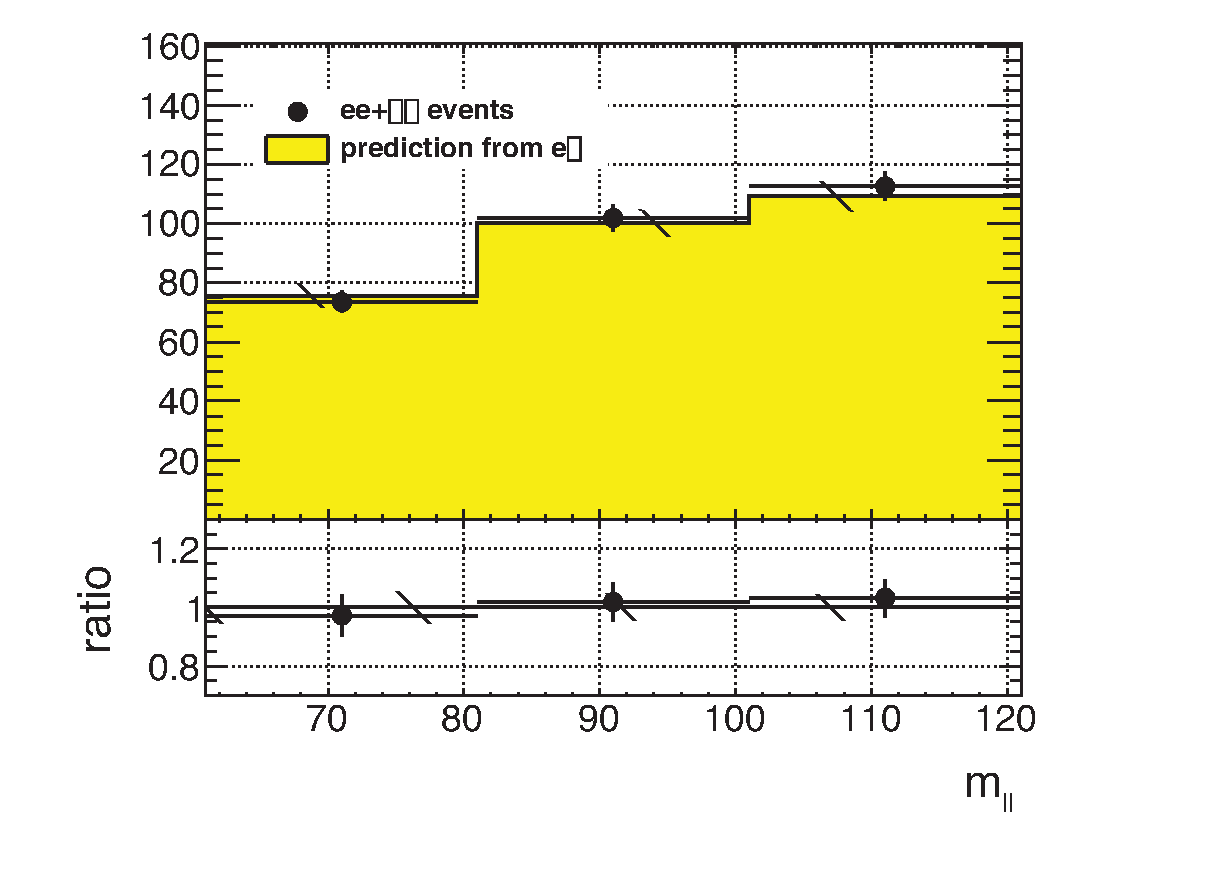
\includegraphics[width=.85\linewidth]{figures/fs/ee+mm_ratio_mll_VRZ_widened.eps}
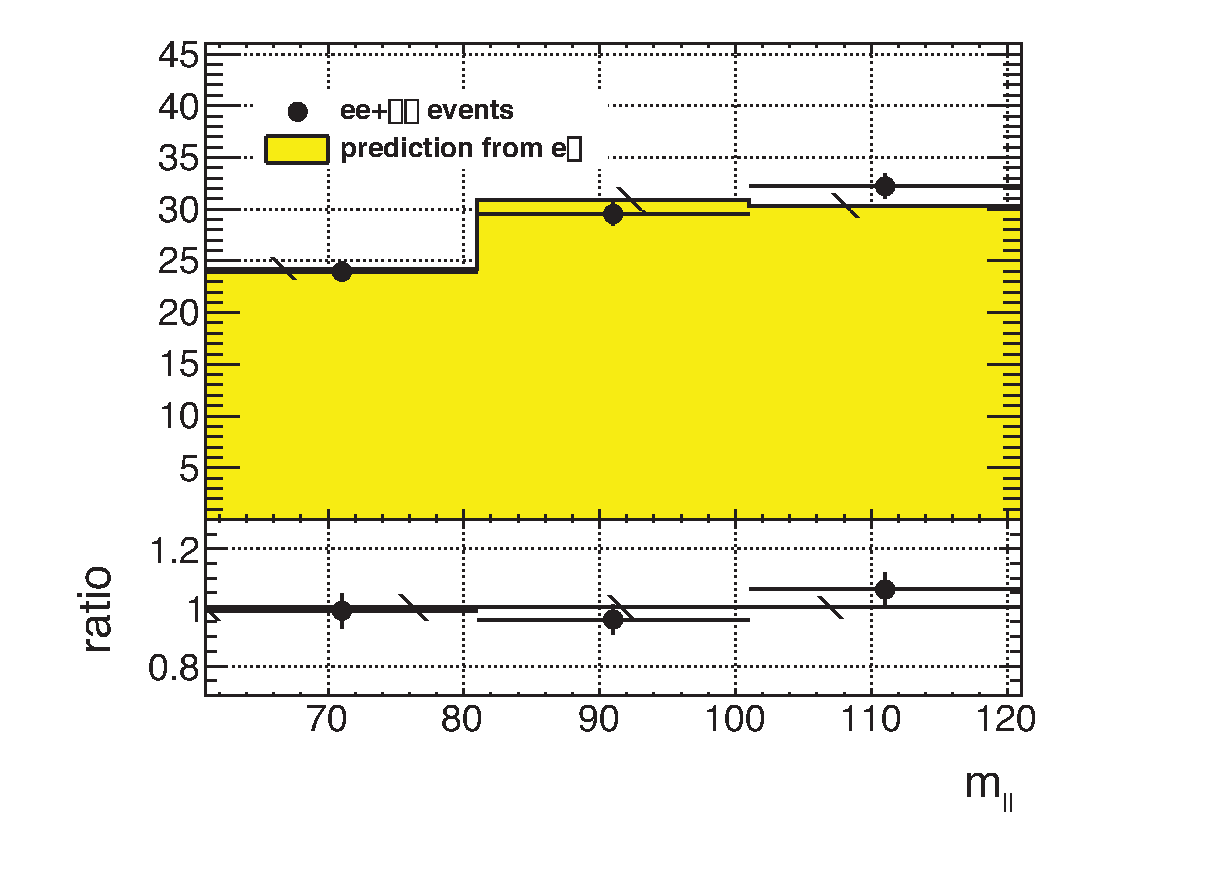
\includegraphics[width=.85\linewidth]{figures/fs/ee+mm_ratio_mll_SRZ_widened.eps}
\caption{\ac{MC} closure plots of VRS (top) and SRZ (bottom). The number of events from MC (black points) is compared to the number of events predicted from the flavor symmetry method (yellow histogram). The comparison is performed before the expanded \mll~window is used to predict the on-$Z$ bin, but because the shape is taken from the same \ac{MC}, the result is identical.}
\label{fig:fs_closure}
\end{figure}
\end{centering}

A small uncertainty is added based on the statistical uncertainty on the $k$ and $\alpha$ factors derived from data. These factors are measured in many different bins (see, for example, the different measurements of $k$ in \autoref{fig:fs_k}), and as a consequence, some bins can have very large statistical uncertainties. To assess the uncertainty on the total estimate, each measurement of these factors is varied by its uncertainty in order to produce the maximum and minimum possible prediction. The differences with respect to the nominal prediction are used to create a symmetrized error, which is included in \autoref{tab:fs_errors}.

\begin{centering}
\begin{figure}[!hbt]
\myfloatalign
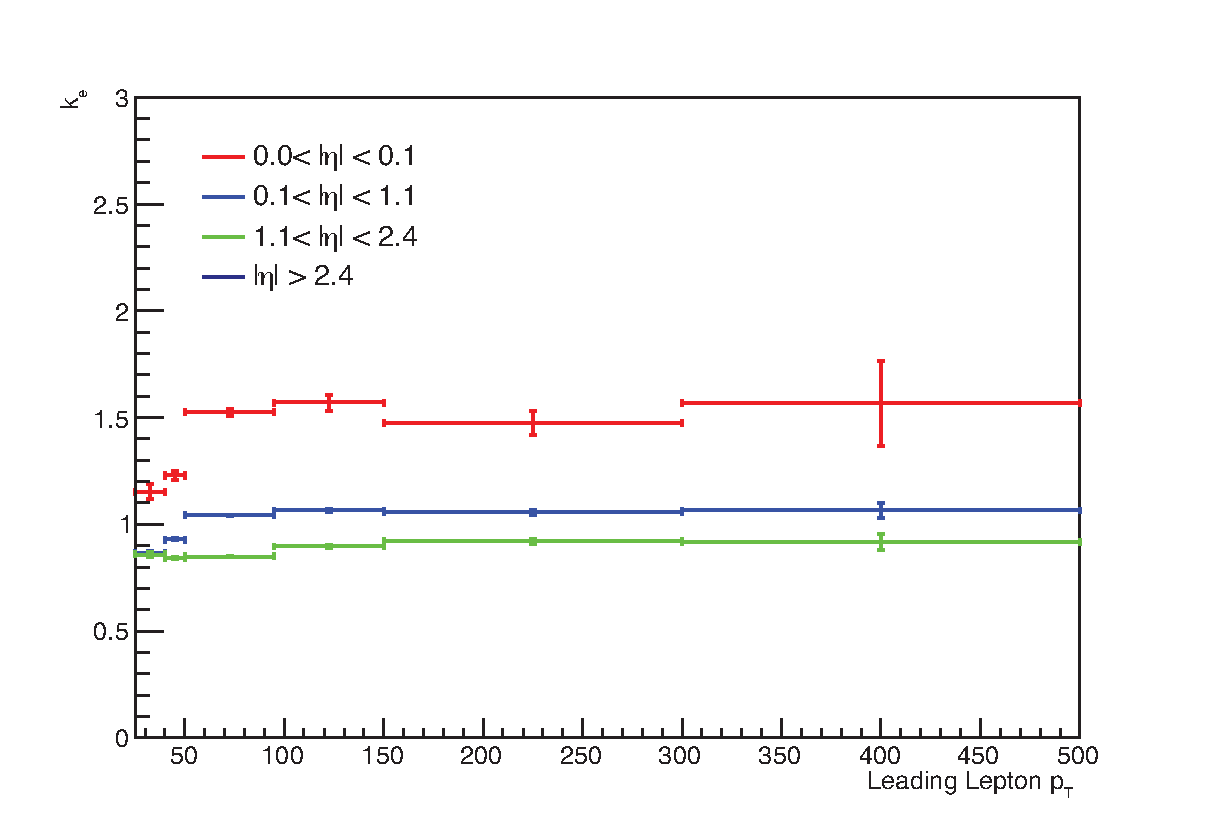
\includegraphics[width=.85\linewidth]{figures/fs/data_efficiencies_2j_Z_lep0.eps}
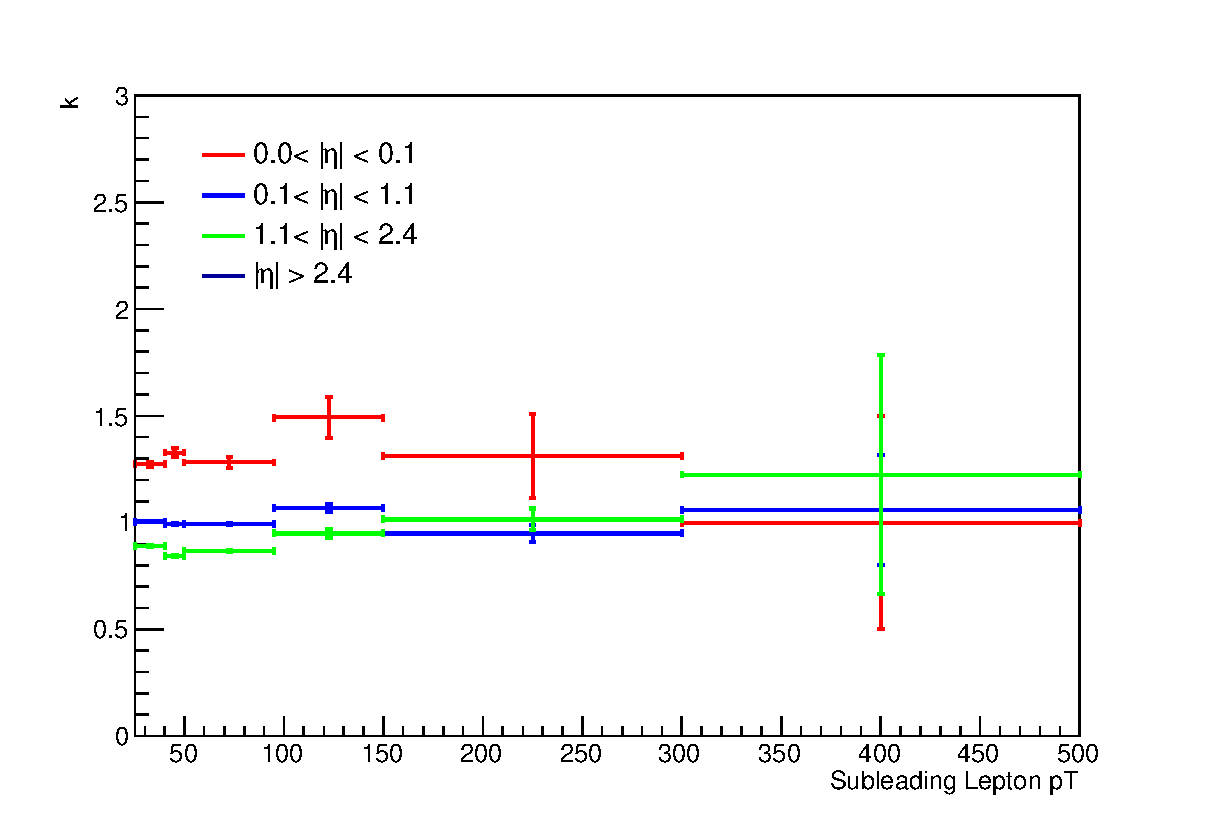
\includegraphics[width=.85\linewidth]{figures/fs/data_efficiencies_2j_Z_lep1.eps}
\caption{Measurements of $k$, the ratio of electron to muon events, in bins of $\pT$ and $\eta$. On the top is the measurements indexed by the leading lepton, while the measurements indexed by the subleading lepton are on the bottom. These efficiencies are for the 2016 dataset.}
\label{fig:fs_k}
\end{figure}
\end{centering}

The next uncertainty considers a potential bias in the way the $\alpha$ factors are calculated. Because they are derived from data, there is already trigger dependence in data collection; only events passing a trigger are stored. Additional trigger dependence is created by the data format used for analysis. ATLAS data and \ac{MC} are stored in a format called \ac{AOD}, but smaller, slimmer versions of these datasets, called \acp{dAOD} are used for analysis. These \acp{dAOD} are designed with specific analyses in mind, filtering on the triggers and objects required by the analyses. As a consequence, in the \ac{dAOD} used in this analysis, there are explicit requirements that lepton or \met triggers are passed in order for events to be included. 

As a consequence, the trigger efficiencies $\epsilon^\text{trig}$ used in \autoref{eq:kandalpha} to define $\alpha$ do not consider all possible data events. The $epsilon^\text{trig}$ factor is calculated for each trigger using events passing the kinematic selection for that trigger, outlined in \autoref{sec:trig_strategy}. The efficiency factor is then measured according to the equation

\begin{equation}
\epsilon^\text{trig} = \frac{N_\text{trig}}{N_\text{all}} 
\end{equation}

where $N_\text{trig}$ is the number of events passing the trigger in the kinematic selection and $N_\text{all}$ is all events in the selection. The latter measurement is the one subject to this bias, as it contains only the events that pass at least one trigger required for inclusion in the \ac{dAOD}. As a consequence of these missing events, the $\epsilon^\text{trig}$ values will be artificially high. However, because the ratio of trigger efficiencies for the different channels is the only quantity needed for this analysis, the missing events will only bias the prediction if the different channels are differently impacted by the trigger preselection.

Calculating the flavor symmetry method's dependence on these biases requires the use of \ac{MC}. With a generated \ac{MC} sample, there is no trigger dependence, so an unskimmed sample can be compared to a typical skimmed \ac{MC} \ac{dAOD} to identify the effect of the skimming. \autoref{fig:fs_alpha} shows a comparison of the $\alpha$ factors calculated for different bins in \met from the nominal source, data, as well as these two \ac{MC} sources. A \met dependence would be the most likely bias between the two \ac{MC}-derived $\alpha$ factors because \met triggers are the only triggers besides lepton triggers that will allow an event to be accepted into the dAOD used by this analysis. Though there is some difference between the data-derived $\alpha$ and those taken from \ac{MC}, it is clear from this plot that there is very little dependence on the choice of an unskimmed or skimmed sample. The calculation of the uncertainty is performed by repeating the flavor symmetric method in \ac{MC} with each of the two $\alpha$ factors and using the difference between the estimates as a symmetric error.

\begin{centering}
\begin{figure}[!hbt]
\myfloatalign
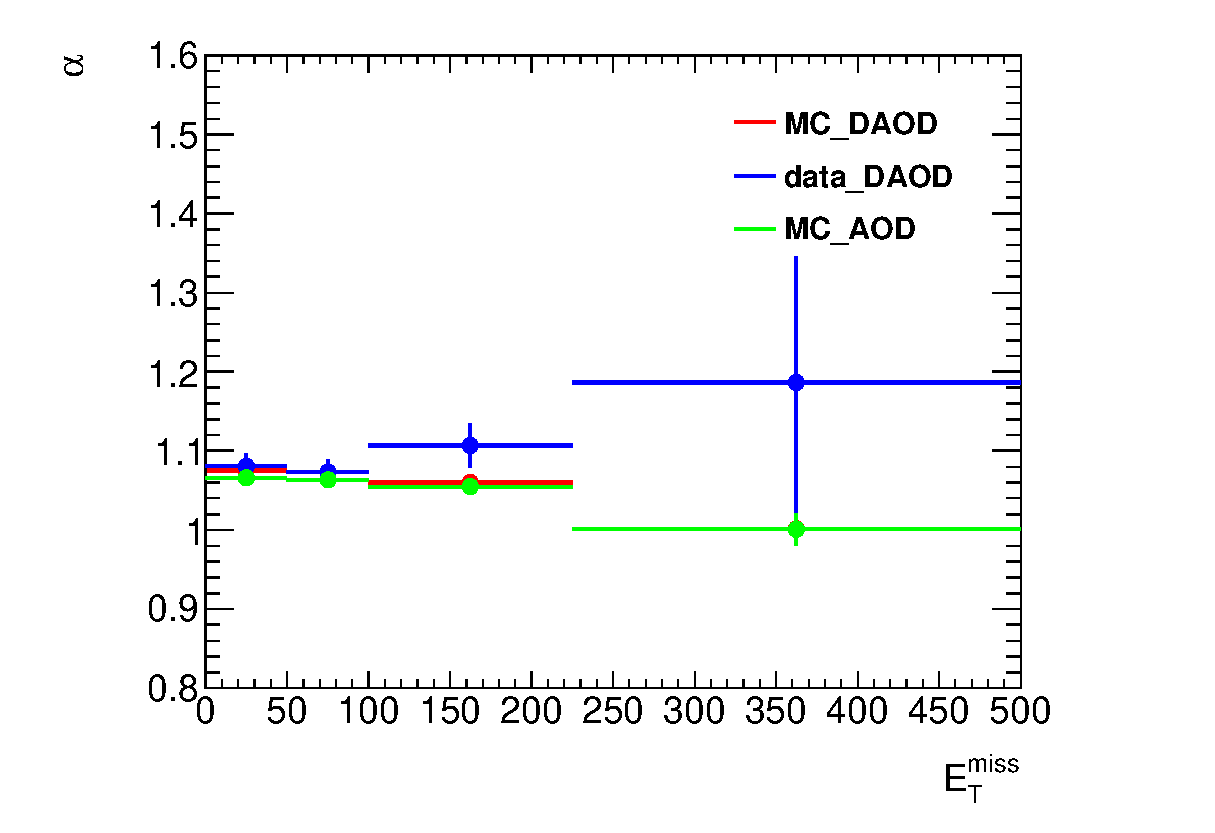
\includegraphics[width=.85\linewidth]{figures/fs/trigger_ratios.eps}
\caption{$\alpha$, the trigger efficiency ratio, calculated as a function of \met from three different sources: data (blue), the usual skimmed \ttbar \ac{MC} (red), and an unskimmed \ttbar \ac{MC} (green).}
\label{fig:fs_alpha}
\end{figure}
\end{centering}

The last uncertainty relates to the main \ac{MC} dependence of the method - the \mll~shape of the \ac{FS} background. A correction factor is taken from \ac{MC} in order to account for the \mll~widening, and the accuracy of that factor must be checked. Its shape is compared to that of data in region similar to VR-FS, but with an \HT cut lowered to 300 \gev~to increase statistics. The difference between the fraction of events on the $Z$-mass peak in data and \ac{MC} in this region is taken as a systematic uncertainty. To confirm that using this lowered \HT cut still gives a valid answer, the fractions are compared as a function of \HT in \autoref{fig:fs_frac_ht}. In these plots, especially in the higher-statistics 2016 plot, it is clear both that the data and \ac{MC} agree very well and that there is no strong \HT dependence. 

\begin{centering}
\begin{figure}[!hbt]
\myfloatalign
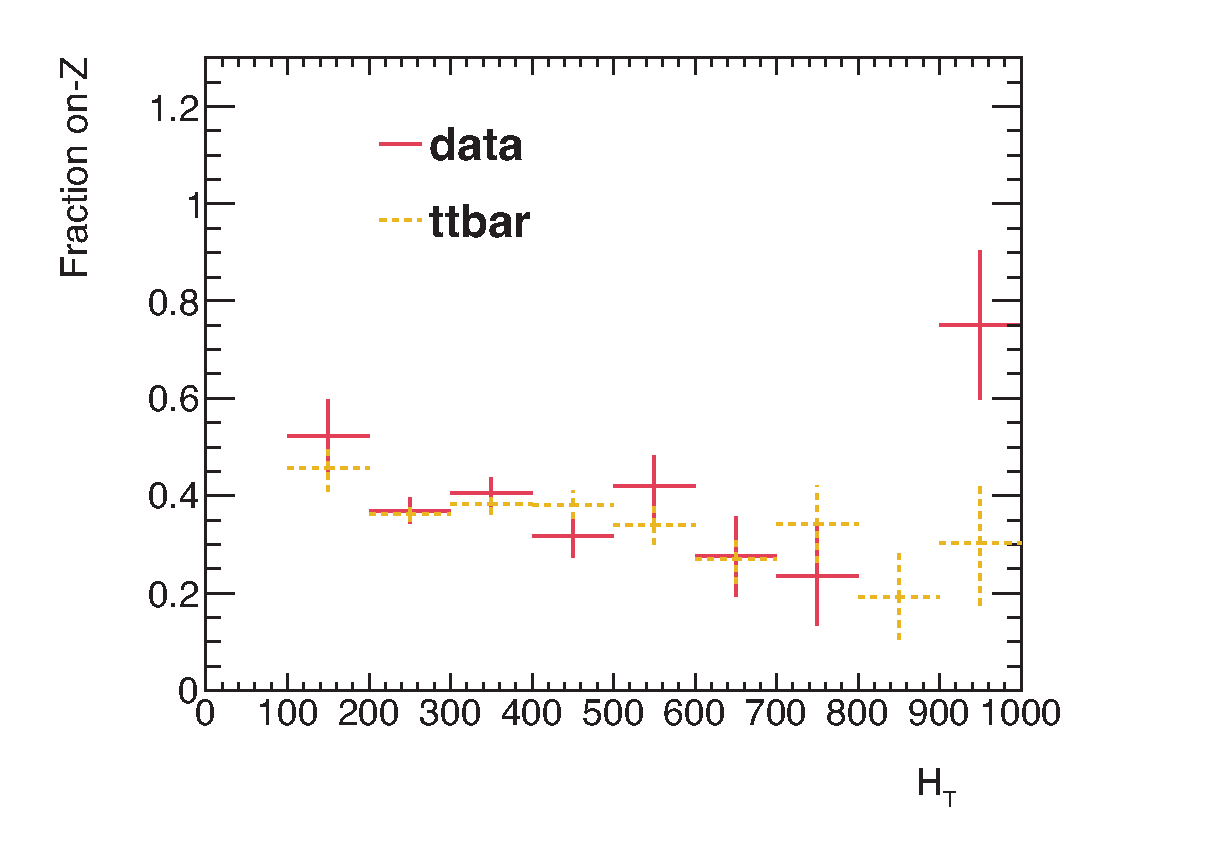
\includegraphics[width=.85\linewidth]{figures/fs/frac_vs_ht_2015.eps}
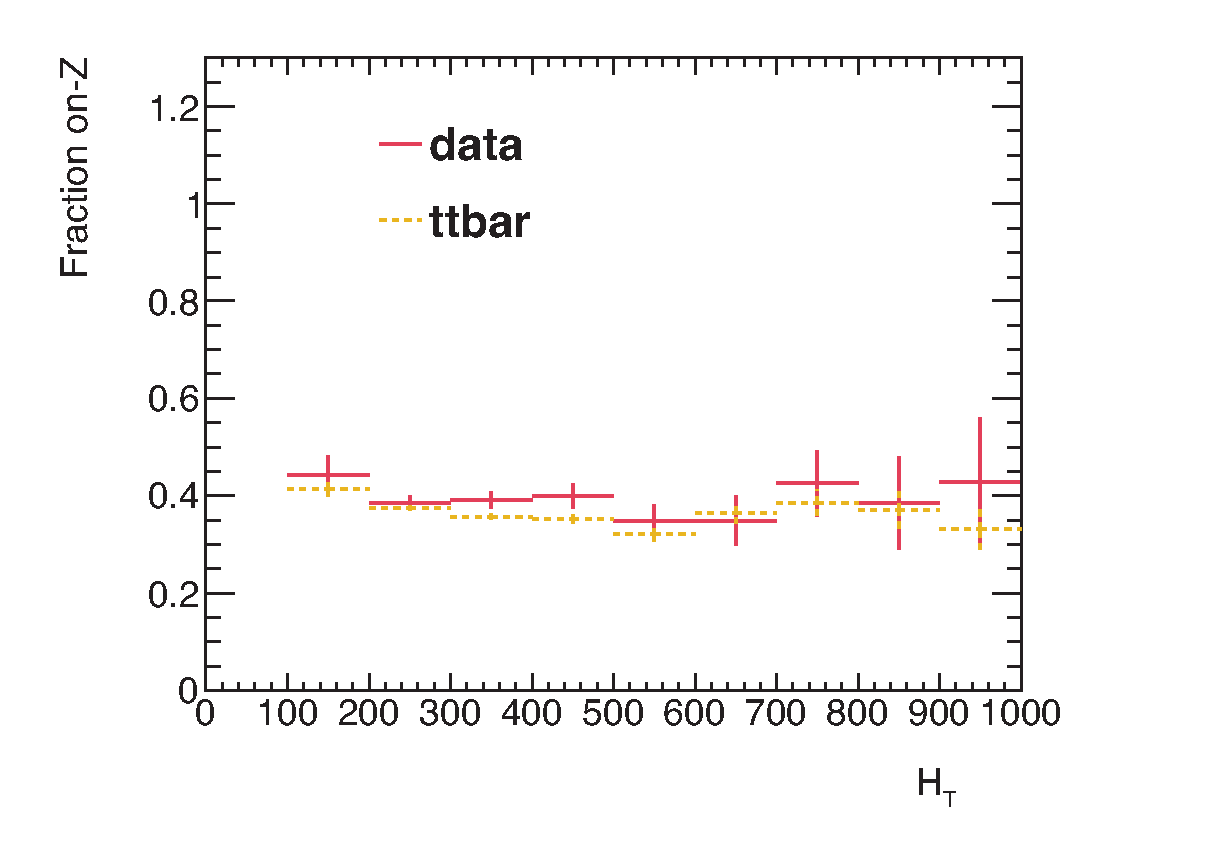
\includegraphics[width=.85\linewidth]{figures/fs/frac_vs_ht_2016.eps}
\caption{Plots of the fraction of on-Z events with a VR-FS-like selection as a function of \HT. The top figure shows 2015 data and \ac{MC} while the bottom figure shows the same for 2016.}
\label{fig:fs_frac_ht}
\end{figure}
\end{centering}

All the uncertainties are calculated independently for the two datasets, then added together. Statistical uncertainties, including the \ac{MC} closure statistical uncertainties and the $k$ and $\alpha$ uncertainties, are added in quadrature between the two years. Uncertainties that are more likely to be correlated, such as the difference between the two estimates in \ac{MC} closure and the dependence on using a dAOD to calculate trigger efficiencies, are added linearly. The total uncertainty is about 12\% of the nominal prediction in SRZ and about 9\% in VRS. 

%----------------------------------------------------------------------------------------

\subsection{Uncertainties on the \gjets Method}

One of the largest sources of uncertainty on the \gjets method is derived by comparing the results from reweighting in different variables. Though boson \pt is used as the nominal reweighting variable, the differences in the kinematics of $\gamma$ and $Z$ events also impact number of jets, \HT, and $E_{\text{T}}$ (which includes the mass of the boson). The \gjets method is repeated using each of these variables to reweight, and their \met distributions are shown in \autoref{fig:photons_rwunc}. The maximum difference from the nominal prediction is symmetrized and used as an uncertainty on the method. 

\begin{centering}
\begin{figure}[bth]
\myfloatalign
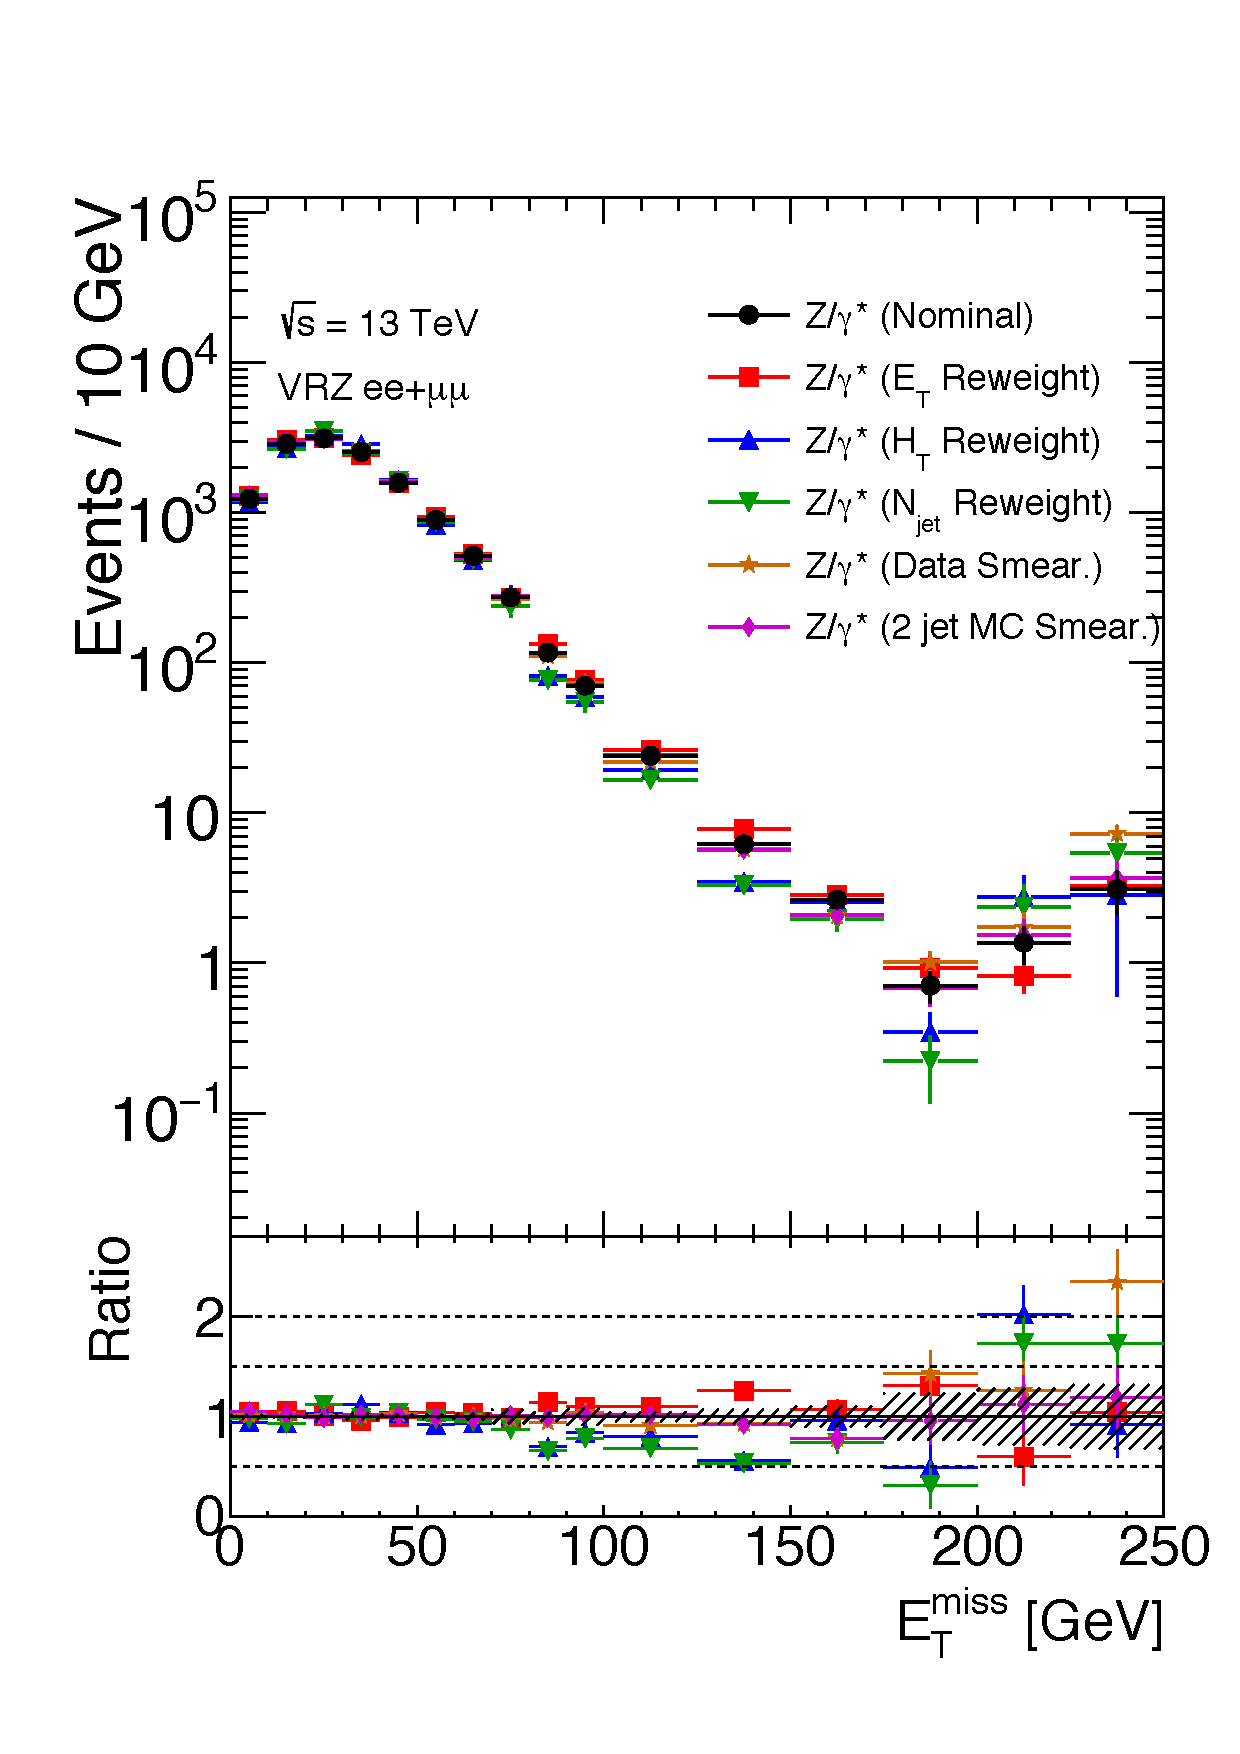
\includegraphics[width=.85\linewidth]{figures/photons/GJ_Variations_ee+mm_zmet_onz.pdf}
\caption{\met distributions for \gjets predictions using different reweighting variables, as well as distributions with the nominal reweighting but with smearing functions taken from data and from \ac{MC} in a $\geq$2-jet region.}
\label{fig:photons_rwunc}
\end{figure}
\end{centering}

Another uncertainty is applied to estimate the validity of using \ac{MC} in a 1-jet \ac{CR} to determine the smearing functions. Smearing functions are made using data from the same 1-jet region and using \ac{MC} in a $\geq$2-jet region otherwise identical to the 1-jet \ac{CR}. These distributions are also shown in \autoref{fig:photons_rwunc}, and like the alternate reweighting distributions, are used to find a maximum difference from the nominal prediction which is translated into a symmetric error. 

As in the flavor symmetric method, the full procedure is carried out on \ac{MC} in order to test \ac{MC} closure, including a recalculation of any weights that are typically derived from data. The resulting comparison between \dyjets \ac{MC} and the \gjets method performed on \ac{MC} can be seen in \autoref{fig:photons_mcclos}. The final non-closure uncertainty is taken from VRS, where larger numbers of events give a clearer picture of the success of the method than in SRZ. In this region, the statistical uncertainty on the prediction is compared to the non-closure, and the larger of the two is used as the final uncertainty. 

\begin{centering}
\begin{figure}[!hbt]
\myfloatalign
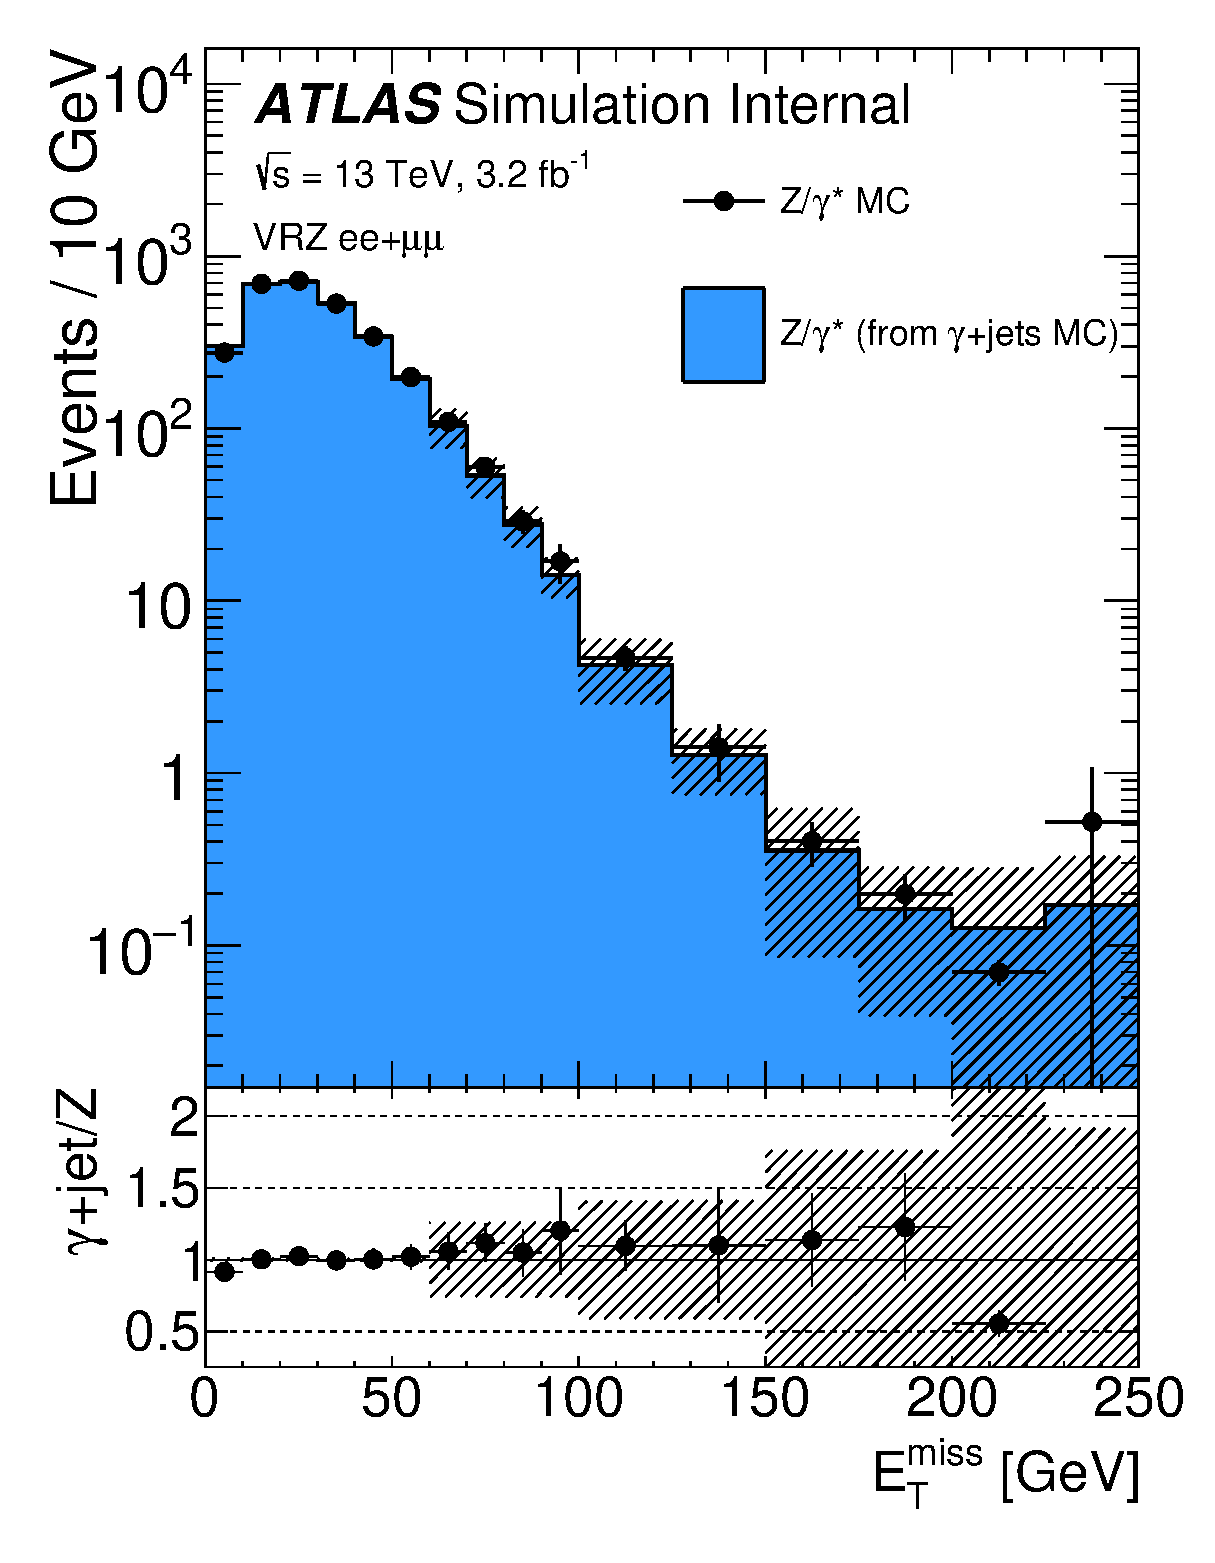
\includegraphics[width=.85\linewidth]{figures/photons/gamma_jet_closure_ee_mm.eps}
\caption{\ac{MC} closure of the \gjets method as a function of \met comparing the \ac{MC} prediction of the $Z$ background with the \gjets method performed on \gjets \ac{MC}. The uncertainty band includes both statistical and reweighting uncertainties.}
\label{fig:photons_mcclos}
\end{figure}
\end{centering}

The uncertainty on the $V\gamma$ contamination in CR-$\gamma$ is also considered. An uncertainty on the \ac{MC} prediction is made based on comparison of data and \ac{MC} in a $W +$ jets \ac{VR}, shown in \autoref{fig:photons_vgunc}. This \ac{VR} is similar to CR-$\gamma$, but instead of vetoing events with leptons, requires at least one well-isolated lepton with a \pt over 25 \gev. At \met values over 100 \gev, region is about 90\% pure in $W\gamma$ processes. The \ac{MC} agrees well with data in this region, even at very high \met, so an uncertainty of 16\% based primarily on statistical uncertainty in this \ac{VR} is placed on the $V\gamma$ \ac{MC}. This uncertainty is propagated to the final result through the subtraction procedure.

\begin{centering}
\begin{figure}[!hbt]
\myfloatalign
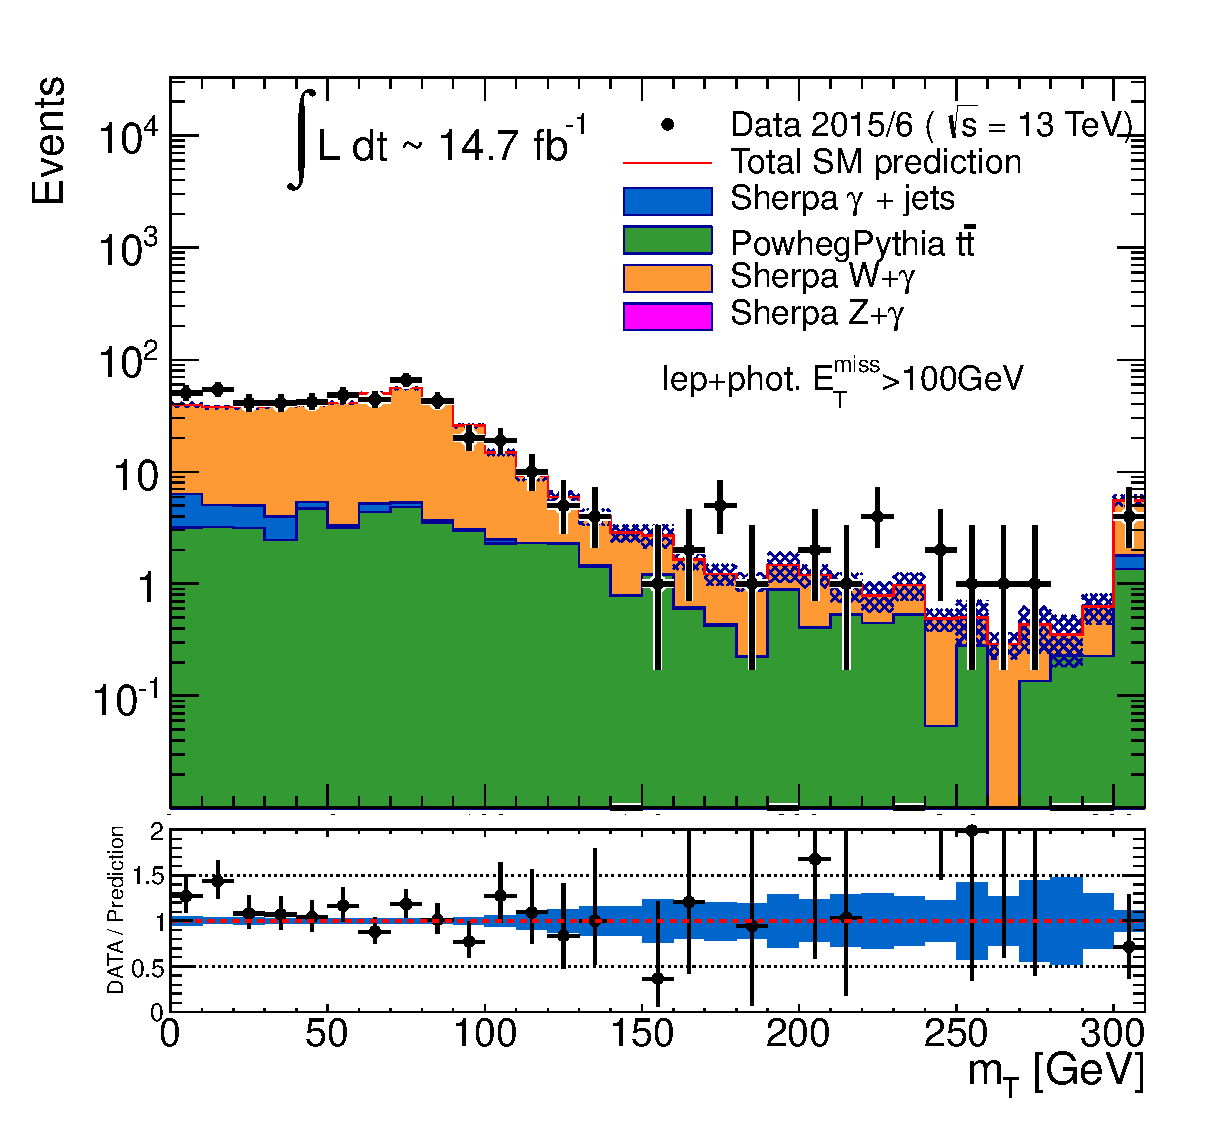
\includegraphics[width=.9\linewidth]{figures/photons/hPhotLep_mT_MET100_hist.eps}
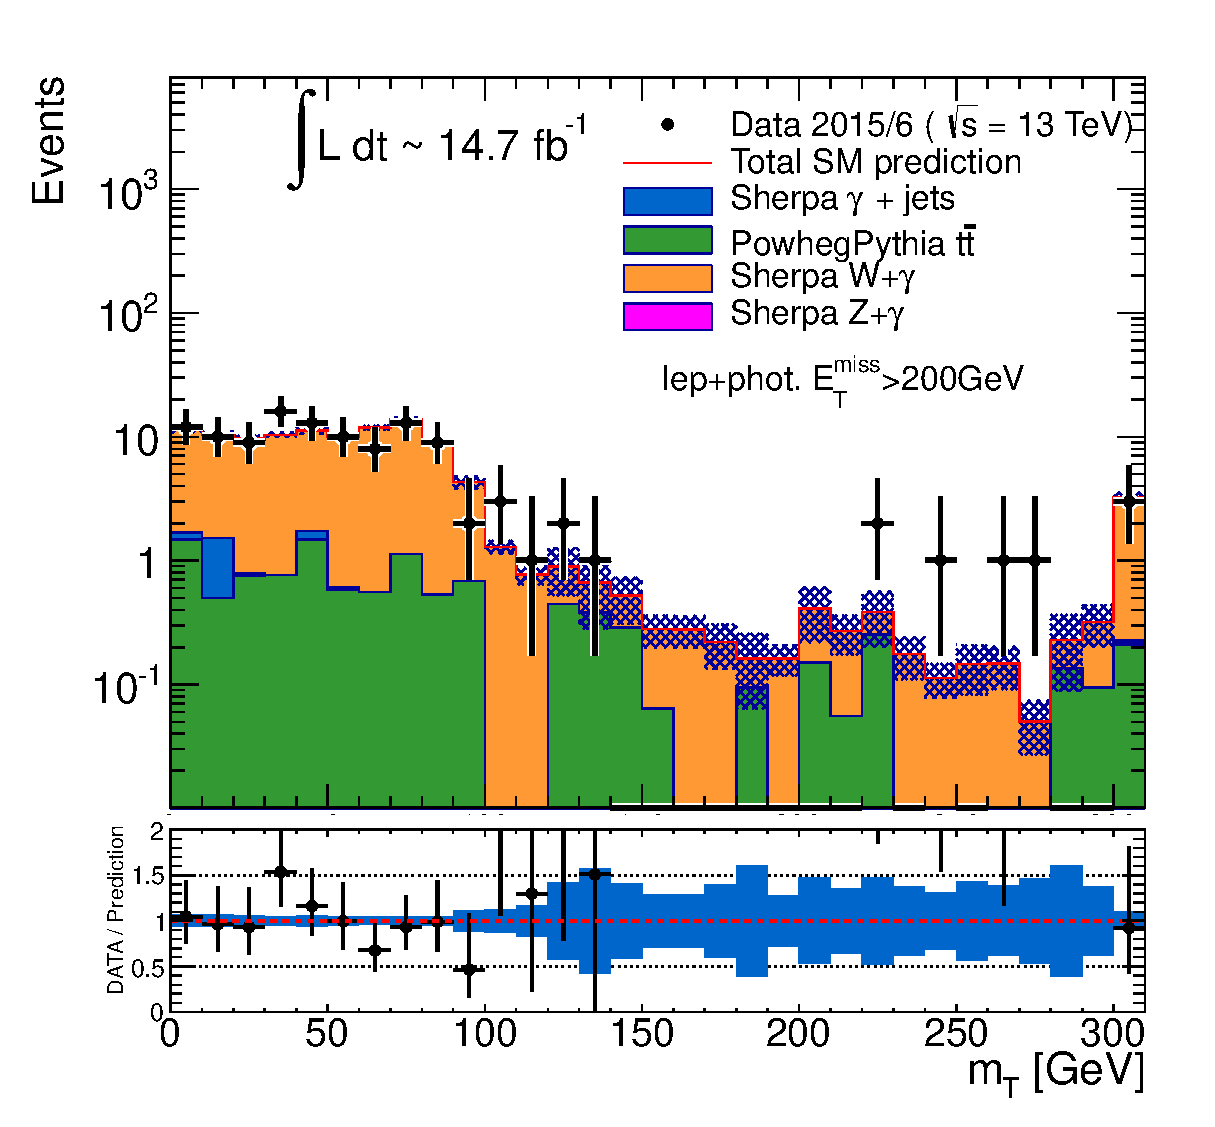
\includegraphics[width=.9\linewidth]{figures/photons/hPhotLep_mT_MET200_hist.eps}
\caption{Distributions of $m_{\text{T}}(\ell,\met)$, the transverse mass of the lepton and the \met in a \ac{VR} designed to target $W\gamma$ processes. Top is the distribution with a \met cut at 100 \gev, and bottom is the same distribution with a \met cut of 200 \gev.}
\label{fig:photons_vgunc}
\end{figure}
\end{centering}

An uncertainty on the \mll~shape is determined using \ac{MC} closure as well. The comparison of \mll~shapes in \dyjets \ac{MC} and the \gjets method applied to \ac{MC} is shown in \autoref{fig:photon_mll_mc}. As with the main \ac{MC} closure test, the maximum of the statistical uncertainty and the non-closure is taken as the final uncertainty on this background.

One last uncertainty based on the statistical uncertainty on the number of \gjets data events used for this method is also included. The full breakdown of uncertainty in SRZ can be seen in \autoref{tab:photon_uncertainties}.

\begin{table}[!hbt]
\centering
\resizebox{\textwidth}{!}{

 \begin{tabular}{cc|ccccccc}
 \hline 
\multirow{3}{*}{Ch.} 	& \multirow{3}{*}{Pred.} & \multicolumn{7}{c}{Uncertainties (\%)} \\
   \cline{3-9} 
   		 	& 	  		& $V\gamma$ 	& MC  		& \mll 	& re- 		& smear  & stat.  	& total \\
   			& 		 	& sub. 			& clos.		& shape & weight	& 		 & 	 		& \\
   \hline
   \hline
$ee$ 			& 1.02 & 53.0 & 21.0 & 19.0 & 100.0 & 65.0 & 56.0 & 145.0 \\ 
$\mu\mu$ 		& 2.08 & 27.0 & 14.0 & 23.0 & 30.0  & 59.0 & 40.0 & 86.0 \\ 
$ee$+$\mu\mu$ 	& 3.1  & 36.0 & 16.0 & 22.0 & 43.0  & 60.0 & 33.0 & 92.0 \\ 
 

\hline
\hline
 \end{tabular}
}
\caption{Uncertainty breakdown for the \gjets method in SRZ. Uncertainties considered are the impact of \ac{MC} uncertainty on $V\gamma$ backgrounds, \ac{MC} closure, uncertainty on \mll shape (also determined via \ac{MC} closure), reweighting uncertainties, smearing uncertainties, and statistical uncertainty on the \gjets events used in the method.}
\label{tab:photon_uncertainties}
\end{table}

%----------------------------------------------------------------------------------------

\subsection{Uncertainties on the Fakes Background}
\label{sec:uncert_fakes}

Systematic uncertainties on the fakes background are derived from a series of variations on the nominal method.  Variations include scaling the real and fake efficiencies up and down by their statistical uncertainties, scaling the prompt lepton contamination in CR-fake up and down by 20\%, and by requiring and vetoing $b$-tagged jets in CR-fake to determine the dependence on heavy flavor. 
Statistical uncertainties can also be large in regions with small numbers of events in the the baseline selection, such as SRZ. In other regions, the $b$-tagging dependence provides the largest uncertainty. The full breakdown of uncertainties for the most important regions are listed in ~\autoref{tab:syst:fakes_onz1516}.

\begin{table}[!hbt]
\centering
\resizebox{\textwidth}{!}{
\begin{tabular}{l|cccccc}
Variation & SRZ & CRT & CRFS & VRFS & VRS & VRT  \\
\hline\hline
Nominal & 0.10 $\pm$ 1.61 & 25.39 $\pm$ 5.35 & 3.73 $\pm$ 2.19 & 10.53 $\pm$ 3.56 & 3.64 $\pm$ 3.20 & 80.06 $\pm$ 9.80   \\
\hline
EL F Up & 0.15  	& 30.23 & 3.96 & 10.93 & 3.56  	& 92.46   \\
EL F Down & 0.06  	& 21.80 & 3.52 & 10.18 & 3.54 	& 70.07   \\
EL R Up & 0.25  	& 26.17 & 3.92 & 11.10 & 4.13 	& 82.57   \\
EL R Down & -0.07  	& 24.51 & 3.52 & 9.92 & 3.10 	& 77.24   \\
MU F Up & -0.20  	& 32.48 & 4.77 & 16.41 & 5.25 	& 86.48   \\
MU F Down & 0.29  	& 20.17 & 2.91 & 7.04 & 2.87 	& 70.12   \\
MU R Up & 0.13 		& 25.67 & 3.78 & 10.66 & 3.81 	& 81.18   \\
MU R Down & 0.05 	& 25.04 & 3.67 & 10.38 & 3.44 	& 78.72   \\
\hline
Total Sys 		& +0.26 -0.35 		& +8.64 -6.39 	& +1.08 -0.87 	& +5.92 -3.56 	& +1.70 -0.97  	& +14.24 -14.42  \\
Total Sys (\%) 	& +261.05 -354.72  	& +34.01 -25.19 & +29.05 -23.23 & +56.22 -33.85 & +46.57 -26.60 & +17.78 -18.02  \\
\hline
Real Cont. Up 	& 0.23 	& 20.97 & 3.06 & 8.08 	& 3.15 	& 68.79   \\
Real Cont. Down & -0.01 & 29.67 & 4.38 & 12.95 	& 4.16 & 90.23   \\
b-jet 			& 0.31 	& 40.44 & 5.28 & 8.98 	& 5.63 & 120.50   \\
no b-jet 		& 0.16 	& 23.44 & 3.08 & 11.38 	& 3.97 & 70.55   \\
\hline
Total Sys & +0.25 -0.11 			& +15.65 -4.83 & +1.69 -0.93 & +2.56 -2.90 & +2.09 -0.49  			& +41.71 -14.74  \\
Total Sys (\%) & +260.46 -109.06 	& +61.66 -19.02 & +45.30 -24.85 & +24.32 -27.58 & +57.31 -13.35 	& +52.10 -18.42  \\
\end{tabular}
}
\caption{ Systematic uncertainties on the fake-lepton background for on-Z regions for 2015+2016 yields. The nominal yield includes statistical uncertainty from the baseline selection in a given region. The following rows indicate the results of varying the real and fake lepton efficiencies up and down by by their statistical uncertainty. Real cont. gives an uncertainty on the the contamination of real leptons in the fake lepton efficiency. $b$-jet and no $b$-jet indicate the impact of requiring or vetoing $b$-tagged jets in the regions used to measure the fake efficiency. \label{tab:syst:fakes_onz1516}}
\end{table}

%----------------------------------------------------------------------------------------

\section{Theoretical and Experimental Uncertainties}

Experimental uncertainties cover any detector effect or \ac{LHC} condition that may not be modeled precisely correctly in \ac{MC}. For each uncertainty, a standard prescription from the ATLAS experiment is followed. Uncertainties are included on the following parameters:  
\begin{itemize}
\item Luminosity (2.9\%) \cite{2011lumi,2012lumi}
\item Jet energy scale \cite{ATL-PHYS-PUB-2015-015}
\item Jet energy resolution \cite{ATL-PHYS-PUB-2015-015}
\item Jet vertex tagging
\item Heavy flavor tagging
\item \met soft term \cite{ATL-PHYS-PUB-2015-023}
\item $e/\mu$ momentum scale  
\item $e/\mu$ trigger, reconstruction, and identification efficiencies
\item Pile-up
\end{itemize}

These uncertainties are applied to all \ac{MC} samples used in the analysis. This includes signal models, diboson and rare top samples for the nominal estimate, and all backgrounds taken from \ac{MC} in the sideband fit. 

Theoretical uncertainties include cross-section uncertainties, scale uncertainties, and \ac{PDF} uncertainties. For the diboson samples, the scale uncertainties, given in \autoref{table:Diboson_theoryuncert} are calculated by varying each scale up and down by a factor of two. These are combined with a 6\% cross-section uncertainty and a generator uncertainty obtained by comparing {\sc Powheg} and {\sc Sherpa} \ac{MC} yields in a given region. This generator uncertainty, shown in \autoref{table:Diboson_powhegsherpa1}, is dominant in most regions. Rare top processes are given a $13\%$ PDF and scale variation uncertainty \cite{Alwall:2014hca} and a $22\%$ cross section uncertainty \cite{Campbell:2012,Lazopoulos:2008,Garzelli:2012bn}. 

\begin{table}
	\begin{center}
 		\begin{tabular}{l|c|c|c|c|c|c|c}
		    \hline \hline 
   			\multicolumn{3}{c}{$VV \rightarrow ll\nu\nu$ Samples} \\
  	 		\hline
			&	SRZ & VRS & CRT & VRT & VRWZ & VRZZ & VR3L \\
			\hline
			resummation & 0.07 & 0.03 & 0.01 & 0.02 & 0.00 & 0.00 & 0.00 \\
			renormalization & 0.13 & 0.17 & 0.16 & 0.22 & 0.00 & 0.00 & 0.00 \\
			factorization & 0.01 & 0.01 & 0.01 & 0.03 & 0.00 & 0.00 & 0.00 \\
			total & 0.15 & 0.17 & 0.16 & 0.22 & 0.00 & 0.00 & 0.00 \\
		    \hline 
   			\multicolumn{3}{c}{$WZ \rightarrow lll\nu$ Samples} \\
  	 		\hline
			&	SRZ & VRS & CRT & VRT & VRWZ & VRZZ & VR3L \\
			\hline
			resummation & 0.07 & 0.05 & 0.13 & 0.08 & 0.02 & 0.00 & 0.01 \\
			renormalization & 0.26 & 0.20 & 0.28 & 0.21 & 0.07 & 0.00 & 0.18 \\
			factorization & 0.04 & 0.04 & 0.02 & 0.06 & 0.01 & 0.00 & 0.02 \\
			total & 0.28 & 0.21 & 0.31 & 0.23 & 0.07 & 0.00 & 0.18 \\
  	 		\hline
   			\multicolumn{3}{c}{$ZZ \rightarrow llll$ Samples} \\
  	 		\hline
			&	SRZ & VRS & CRT & VRT & VRWZ & VRZZ & VR3L \\
			\hline
			resummation & 0.27 & 1.07 & 0.01 & 0.01 & 0.06 & 0.01 & 0.53 \\
			renormalization & 0.28 & 0.26 & 0.30 & 0.60 & 0.07 & 0.04 & 0.14 \\
			factorization & 0.27 & 0.25 & 0.30 & 0.58 & 0.13 & 0.02 & 0.16 \\
			total & 0.48 & 1.13 & 0.43 & 0.84 & 0.16 & 0.05 & 0.57 \\
  	 		\hline
 		\end{tabular}
	\end{center}
	\caption{Fractional uncertainties of dibosons in signal and validation regions from Sherpa scale variations.}
	\label{table:Diboson_theoryuncert}
\end{table}

\begin{table}
\begin{center}
\begin{tabular}{c|c|c|c|c|c} \\
Region & Sherpa & Sherpa & Powheg & Powheg & \% \\
& Events/fb$^{-1}$ & Events & Events/fb$^{-1}$ & Events & Difference \\
\hline
\hline
\multicolumn{6}{c}{WZ Samples} \\
\hline
SRZ+VRZ & 5.219 & 76.722 & 3.286 & 48.300 & 37.046 \\
CRT+VRT & 1.060 & 15.583 & 0.742 & 10.913 & 29.970 \\
\hline
\multicolumn{6}{c}{WW/ZZ Samples} \\
\hline
SRZ+VRZ & 1.921 & 28.244 & 0.685 & 10.070 & 71.424 \\
CRT+VRT & 6.281 & 92.332 & 3.142 & 46.188 & 55.474 \\
\hline
\end{tabular}
\end{center}
\caption{Comparison of yields in on-$Z$ and off-$Z$ regions in Sherpa and Powheg diboson MC at $14.7~\mathrm{fb}^{-1}$.}
\label{table:Diboson_powhegsherpa1}
\end{table}

Signal models have both the central value and uncertainty on cross-sections taken from an envelope of predictions using different scales and \ac{PDF} sets \cite{Kramer:2012bx}. The signal processes are calculated at \ac{NLO+NLL}; they are initially callculated at \ac{NLO} in the strong coupling constant, with additional terms from next-to-leading-logarithmic resummation of soft gluon emission \cite{Beenakker:1996ch,Kulesza:2008jb,Kulesza:2009kq,Beenakker:2009ha,Beenakker:2011fu}.


%----------------------------------------------------------------------------------------

\section{Impact of Uncertainties on the Signal Region}


The breakdown of each major uncertainty's contribution to the total uncertainty in SRZ is shown in \autoref{tab:syst}. The dominant uncertainty is the diboson generator uncertainty, followed by the statistical uncertainty from the \ac{FS} background. Uncertainties smaller than 1\% are not shown in the table. 

\begin{table}[h]
\centering
\small
\begin{tabular}{lc}
\noalign{\smallskip}\hline\noalign{\smallskip}
Source  & Relative systematic uncertainty [\%] \\
\noalign{\smallskip}\hline\noalign{\smallskip}
 & SRZ \\
\noalign{\smallskip}\hline\noalign{\smallskip}
Total systematic uncertainty & 17    \\ 
\noalign{\smallskip}\hline
$WZ/ZZ$ generator uncertainty  & 13  \\
Flavour symmetry (statistical) & 7   \\
$WZ/ZZ$ scale uncertainty      & 6   \\
\dyjets\ (systematic)          & 4   \\
Flavour symmetry (systematic)  & 3   \\
\dyjets\ (statistical)         & 2   \\
Fake-leptons                   & 1   \\
\noalign{\smallskip}\hline
\end{tabular}
\caption{
Overview of the dominant sources of systematic uncertainty on the total background estimate in the signal regions.
The values shown are relative to the total background estimate, shown in \%.}
\label{tab:syst}
\end{table}

%----------------------------------------------------------------------------------------